% !TEX TS-program = xelatex
% !BIB TS-program = bibtex
\documentclass[12pt,letterpaper]{article}
\usepackage{style/dsc180reportstyle} % import dsc180reportstyle.sty
\usepackage{float} % for [H] figure placement

%%%%%%%%%%%%%%%%%%%%%%%%%%%%%%%%%%%%%%%%%%%%%%%%%%%%%%%%
%%%% Title and Authors
%%%%%%%%%%%%%%%%%%%%%%%%%%%%%%%%%%%%%%%%%%%%%%%%%%%%%%%%

\title{DSC Capstone Q1 Report}

\author{Jevan Chahal\\
  {\tt j2chahal@ucsd.edu} \\\And
  Hillary Change \\
  {\tt hic001@ucsd.edu} \\\And
  Kurumi Kaneko \\
  {\tt kskaneko@ucsd.edu} \\\And
  Kevin Wong \\
  {\tt kew024@ucsd.edu} \\\And
  Brian Duke \\
  {\tt brian.duke@prismdata.com} \\\And
  Kyle Nero \\
  {\tt kyle.nero@prismdata.com} \\}

\begin{document}
\maketitle

%%%%%%%%%%%%%%%%%%%%%%%%%%%%%%%%%%%%%%%%%%%%%%%%%%%%%%%%
%%%% Abstract and Links
%%%%%%%%%%%%%%%%%%%%%%%%%%%%%%%%%%%%%%%%%%%%%%%%%%%%%%%%

\begin{abstract}
    \textcolor{Black}{
    The process of capturing what makes a creditor trustworthy or not is especially vital within the confines of bank data, due to the guidelines and ethics of what makes this data usable. Although the quantity of the data is massive, there are only a few available features that are explicitly useful in the confines of machine learning, which calls into question how we should measure customer's trustworthiness towards their creditors. Our methodology details the process of refining bank data into categories using Natural Language Processing, assessing individual's income based on bank data alone, and also measuring their credit worthiness both accurately and efficiently. 
    }
\end{abstract}

\begin{center}
Code: \url{https://github.com/hillarychang/dsc180a-capstone-q1}
\end{center}

\maketoc
\clearpage

%%%%%%%%%%%%%%%%%%%%%%%%%%%%%%%%%%%%%%%%%%%%%%%%%%%%%%%%
%%%% Main Contents
%%%%%%%%%%%%%%%%%%%%%%%%%%%%%%%%%%%%%%%%%%%%%%%%%%%%%%%%

\section{Introduction}
Predicting a customer’s creditworthiness is an essential task for banks, as it informs decisions relating to the profitability and risks of loans, credit cards, and other financial services. While traditional credit scores are widely used, they often overlook important aspects of customer behavior, especially for individuals with limited credit history. We aim to develop an alternative approach by analyzing transaction data to create a new creditworthiness measure, which we will call the "Blank Score." By examining patterns in spending, income consistency, and transaction types, we hope to create a model that more accurately reflects individual financial reliability.

\subsection{Data Description}
The dataset, provided by Prism Data, consists of detailed transaction records that include fields such as \texttt{memo}, \texttt{amount}, \texttt{date}, and \texttt{category}.
\begin{itemize}
    \item \textbf{\texttt{prism\_consumer\_id} (Quantitative):} Unique identifier for each consumer, used to analyze spending and income patterns per user.
    \item \textbf{\texttt{prism\_account\_id} (Qualitative):} Identifier for each account, distinguishing multiple accounts for a single consumer or across consumers.
    \item \textbf{\texttt{memo} (Qualitative):} Descriptive text providing transaction details, such as "grocery store" or "ATM withdrawal," useful for categorization.
    \item \textbf{\texttt{amount} (Quantitative):} Transaction value, where positive values represent inflows (e.g., deposits) and negative values represent outflows (e.g., payments).
    \item \textbf{\texttt{posted\_date} (Qualitative):} Date each transaction was posted, enabling temporal analysis of spending trends.
    \item \textbf{\texttt{category} (Qualitative):} Pre-assigned transaction type label, such as "food" or "utilities," serving as a basis for categorization.
\end{itemize}

\subsection{Exploratory Data Analysis}
We first conducted Exploratory Data Analysis using transaction data given to us from our industry partner, Prism Data. This analysis allowed us to identify different patterns. In specific, we observed notable differences in spending behaviors across various time periods. For instance, we noticed that most purchases occurred on weekdays, while weekends had significantly less purchasing priority, suggesting that consumers prioritize certain purchases during the week. 

We also examined seasonal patterns within the dataset, which spans from 2020 to 2023. Certain months, like April and May, showed increased inflows likely due to tax returns, while December exhibited higher spending, likely due to holiday-related expenses. These patterns indicate regular income and expenditure behaviors that could be relevant for predicting creditworthiness.

\begin{figure}[H]
    \centering
    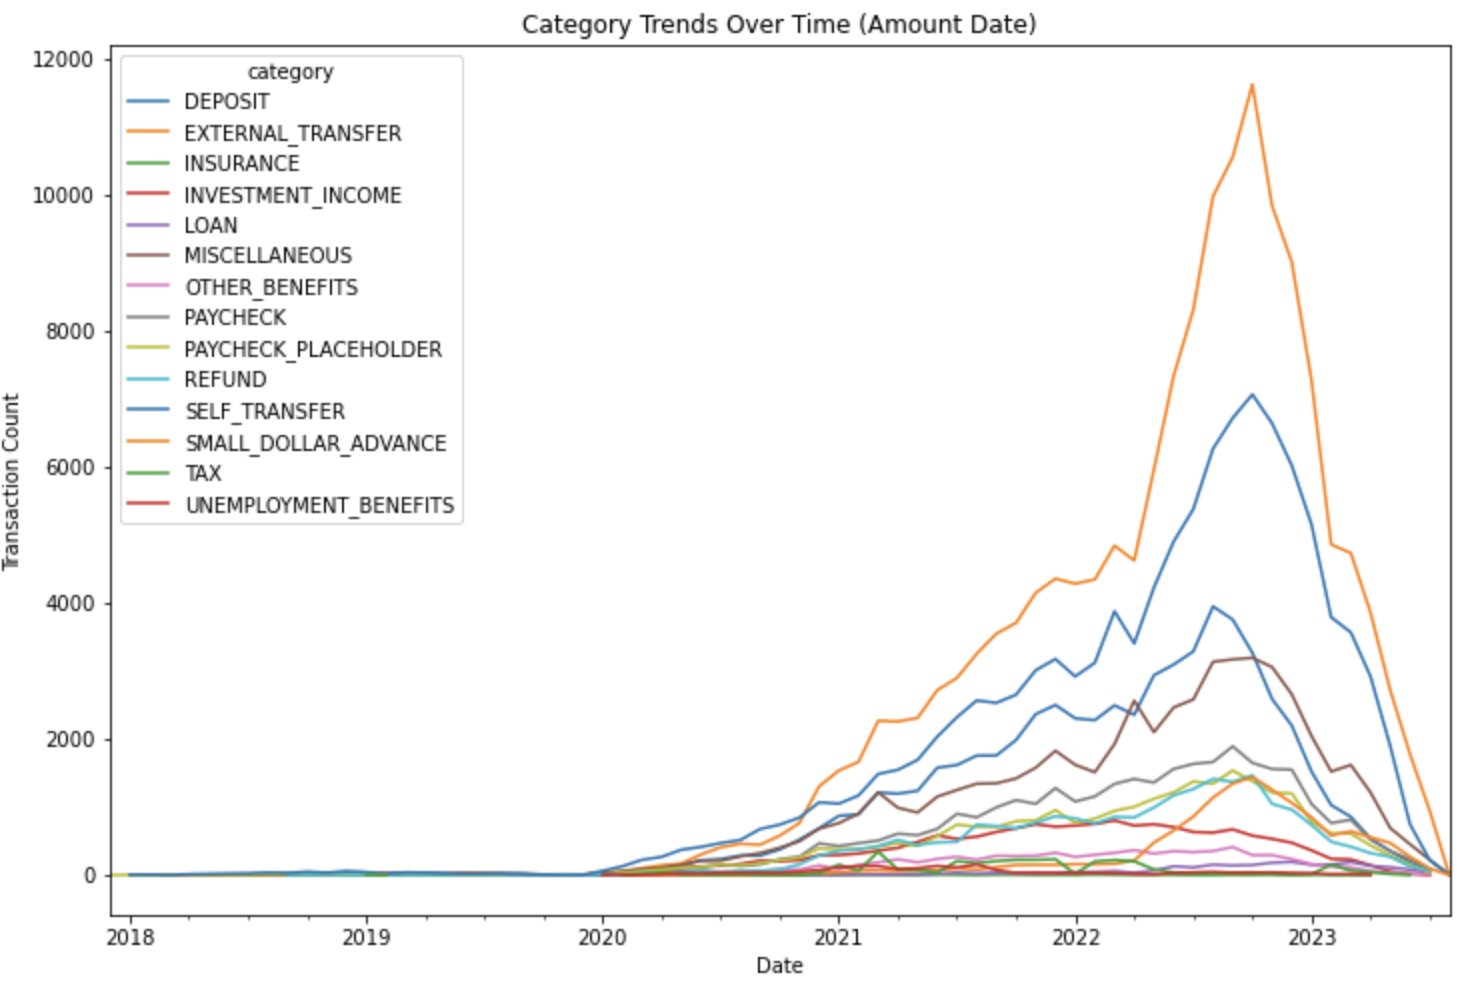
\includegraphics[width=\textwidth]{figure/category_time.png}
    \caption{Trends of transaction categories over time. This exploratory analysis visualizes patterns in transaction volume across different categories, revealing insights such as seasonal spending behavior and category-specific peaks. For example, categories like \texttt{DEPOSIT} and \texttt{EXTERNAL\_TRANSFER} show higher transaction counts in certain months.}
    \label{fig:category_trends}
\end{figure}

\begin{figure}[H]
    \centering
    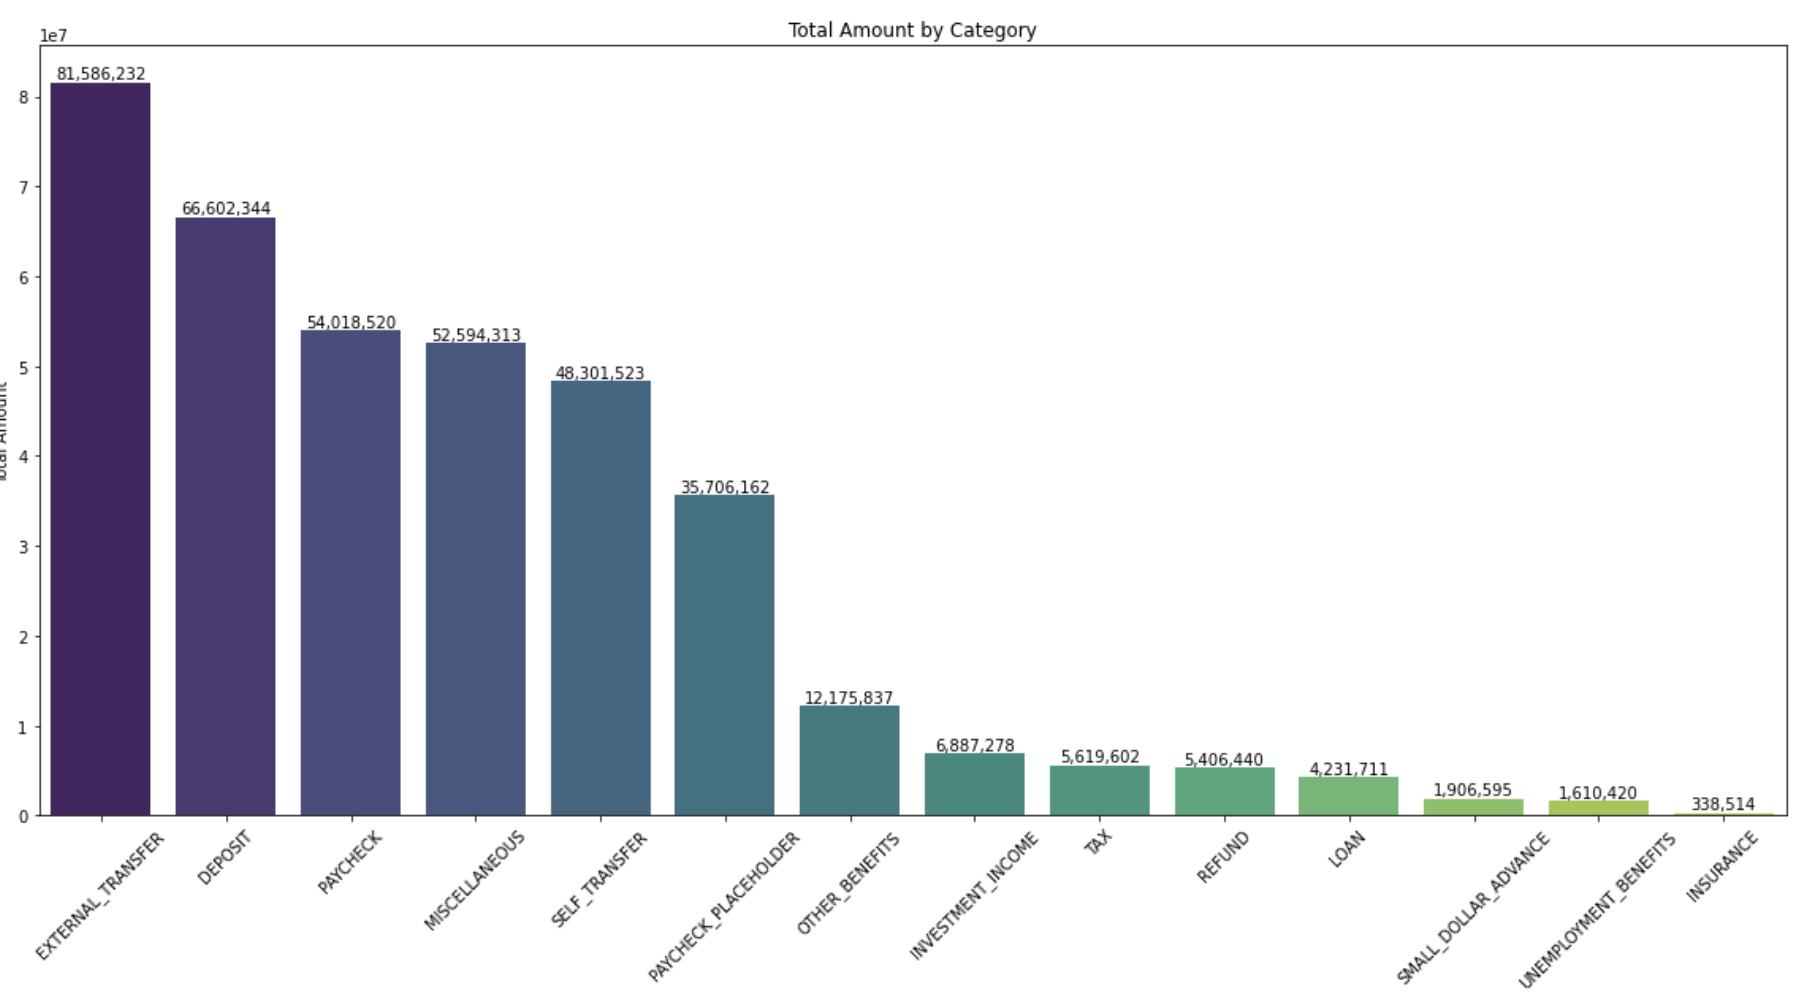
\includegraphics[width=\textwidth]{figure/amt_category.png}
    \caption{Bar chart showing the total amount spent across categories. This visualization highlights which categories contribute the most to overall expenditure, with \texttt{EXTERNAL\_TRANSFER}, \texttt{DEPOSIT}, and \texttt{PAYCHECK} as leading contributors. This information is valuable for understanding the primary financial activities within the dataset.}
    \label{fig:total_amount_by_category}
\end{figure}

\subsection{Train-Test Split and Data Distribution}
\begin{figure}[H]
    \centering
    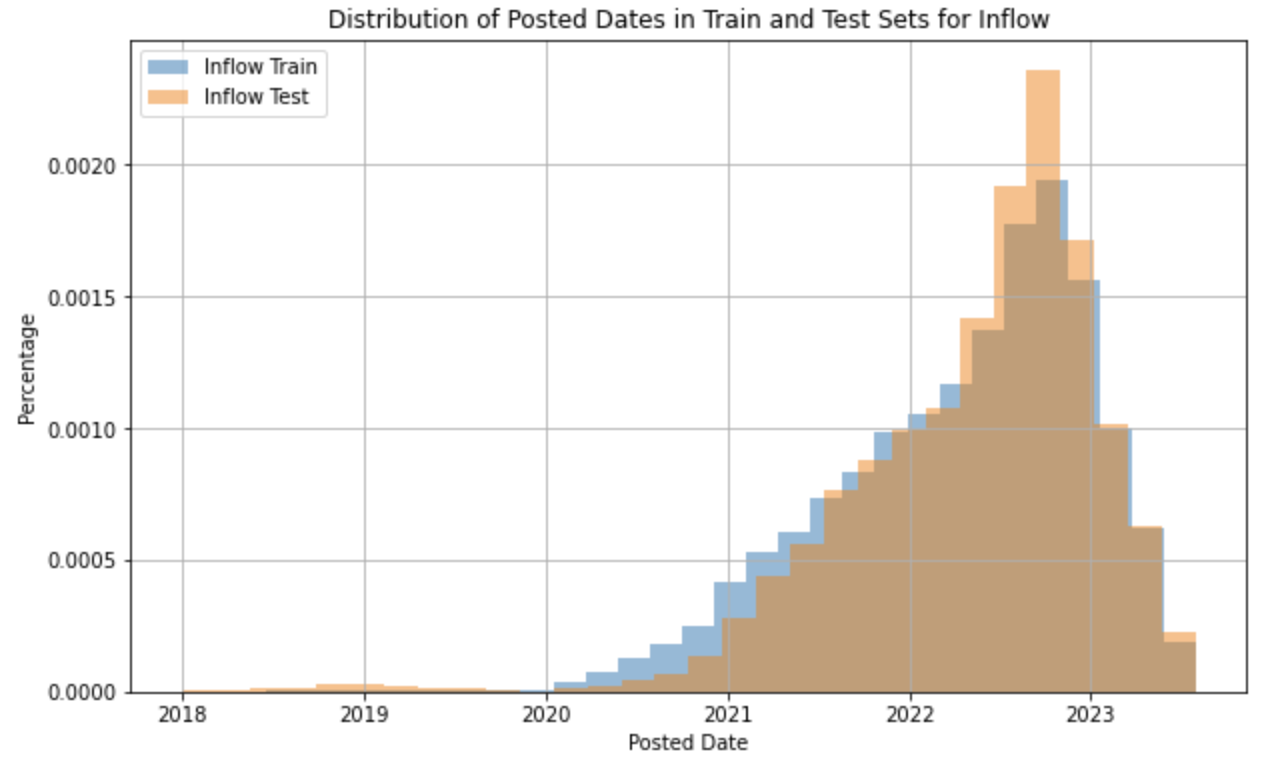
\includegraphics[width=\textwidth]{figure/inflow.png}
    \caption{Histogram of posted dates for the Inflow dataset. The distribution between training and testing sets is almost identical, indicating that the split was performed evenly across time periods. This ensures that both sets are representative of the overall data distribution and reduces potential biases when developing models.}
    \label{fig:inflow_date_distribution}
\end{figure}

\begin{figure}[H]
    \centering
    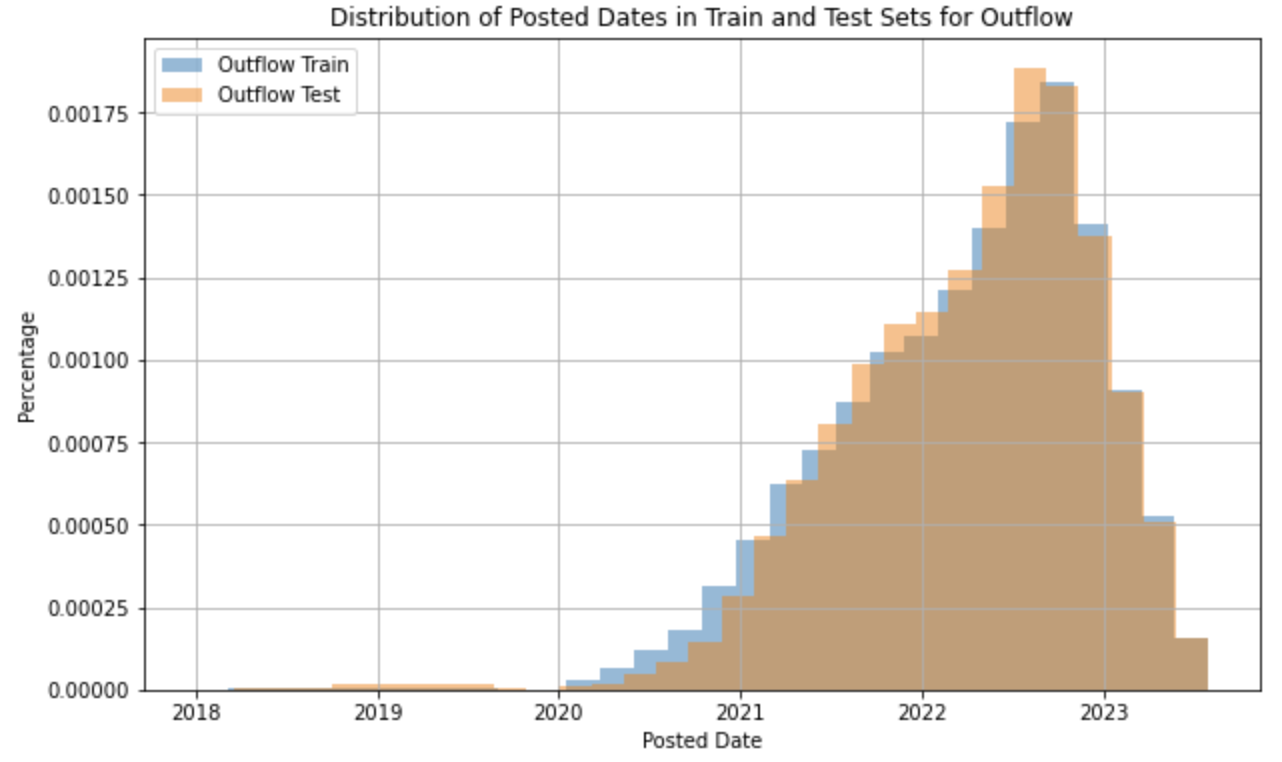
\includegraphics[width=\textwidth]{figure/outflow.png}
    \caption{Histogram of posted dates for the Outflow dataset. Similar to the Inflow dataset, the distribution of dates is balanced between the training and testing sets, verifying an even temporal split. This helps in maintaining consistency and prevents temporal biases in model training and evaluation.}
    \label{fig:outflow_date_distribution}
\end{figure}

\section{Methods}
\subsection{Data Cleaning}
To prepare the memo field for analysis, we first applied a series of cleaning steps to standardize the text. We transformed all text to lowercase for uniformity, removed any extraneous punctuation and symbols, and stripped out dates, state abbreviations, and recurring text that didn’t contribute to transaction categorization (ex., “POS withdrawal”). We also removed placeholder values, such as multiple X’s.

To prepare the dataset for modeling, we began by reviewing a sample of unique transaction memos from each category. This step provided insights into common patterns and inconsistencies, helping us determine the scope and focus of our cleaning tasks.

\begin{figure}[H]
    \centering
    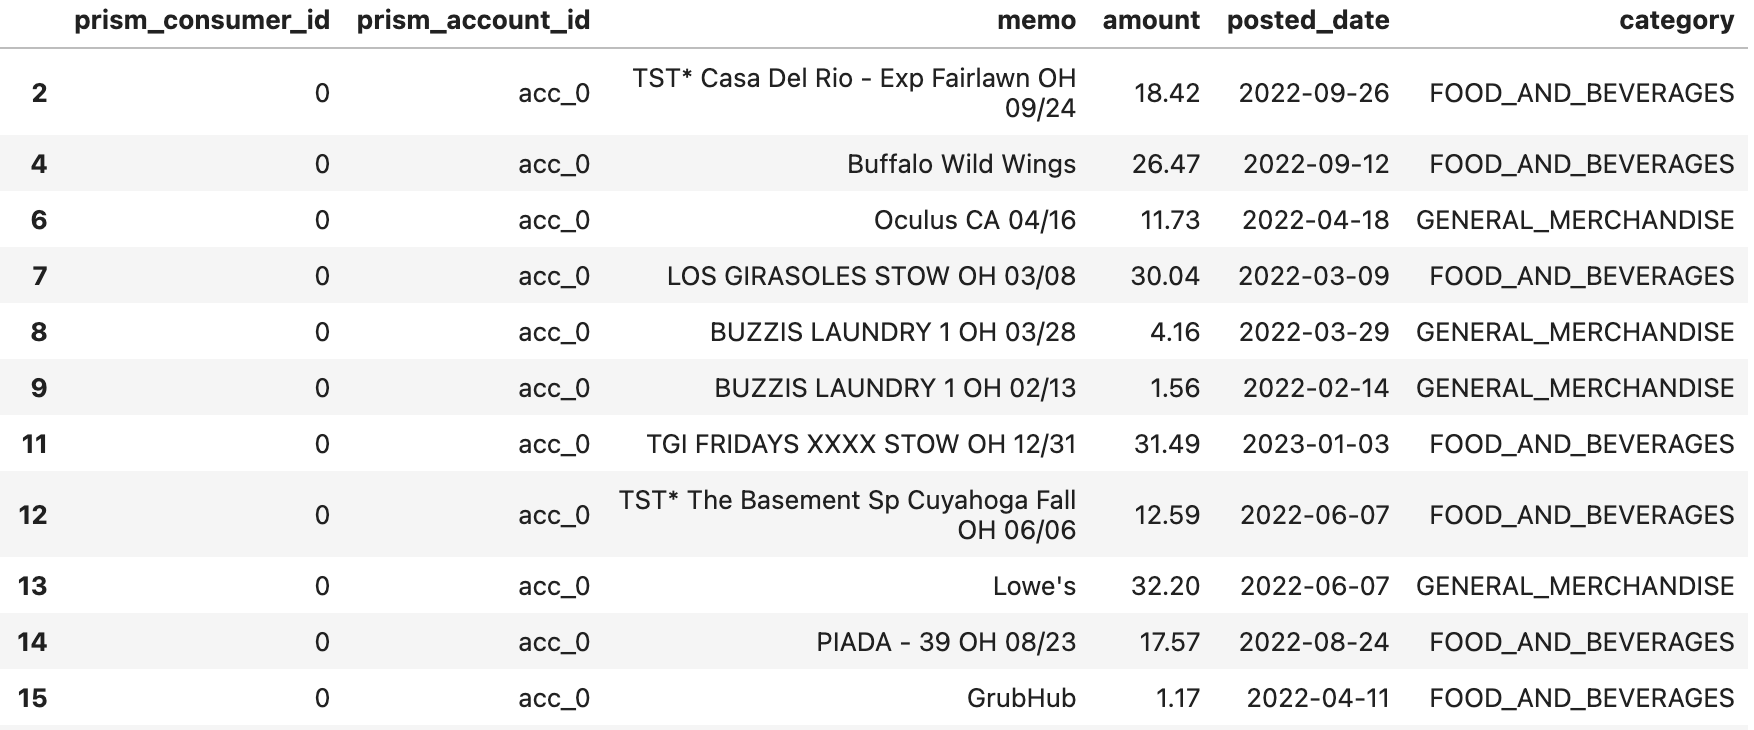
\includegraphics[width=\textwidth]{figure/nonclean_df.png}
    \caption{This table shows the memo dataframe before cleaning. Variations in text format, inconsistent capitalization, and extraneous characters can be observed, which motivated the cleaning process to improve uniformity in transaction descriptions.}
    \label{fig:pre_cleaned_memo}
\end{figure}

We then applied several transformations to standardize the data and improve its interpretability:

\begin{enumerate}
    \item \textbf{Date Removal}: We used regular expressions (RegEx) to locate and remove dates across entries in the memo column, as they did not contribute to the model's predictive goals and added unnecessary complexity. We also removed any extraneous or ambiguous patterns (e.g., “XXXX” entries).

    \item \textbf{Pattern Recognition}: Specific patterns and keywords were identified as indicators of certain transaction categories. For example, "TST" reliably associated with "Food and Beverages," while strings like "APPLE.COM/BILL" were linked to "General Merchandise." We flagged these patterns to automate future classifications and reduce manual intervention.

    \item \textbf{Selective Character Retention}: To preserve potentially valuable information, we retained certain characters such as dots ('.'). This choice allowed us to keep URLs or email addresses within the memo field, which could provide clues to the transaction category.

    \item \textbf{Transaction Labels}: We also identified recurring phrases such as "POS Withdrawal," location-specific markers (e.g., “CA 10/27” for state and date), and labels indicating recurring payments. These were removed for as they did not contribute to the model's predictive goals and added unnecessary complexity.

    \item \textbf{Text Normalization}: All text was converted to lowercase to reduce variability due to case differences.
\end{enumerate}

By implementing these steps, we improved data consistency and ensured key transactional information was preserved, enhancing our model's ability to accurately predict customer creditworthiness.

\begin{figure}[H]
    \centering
    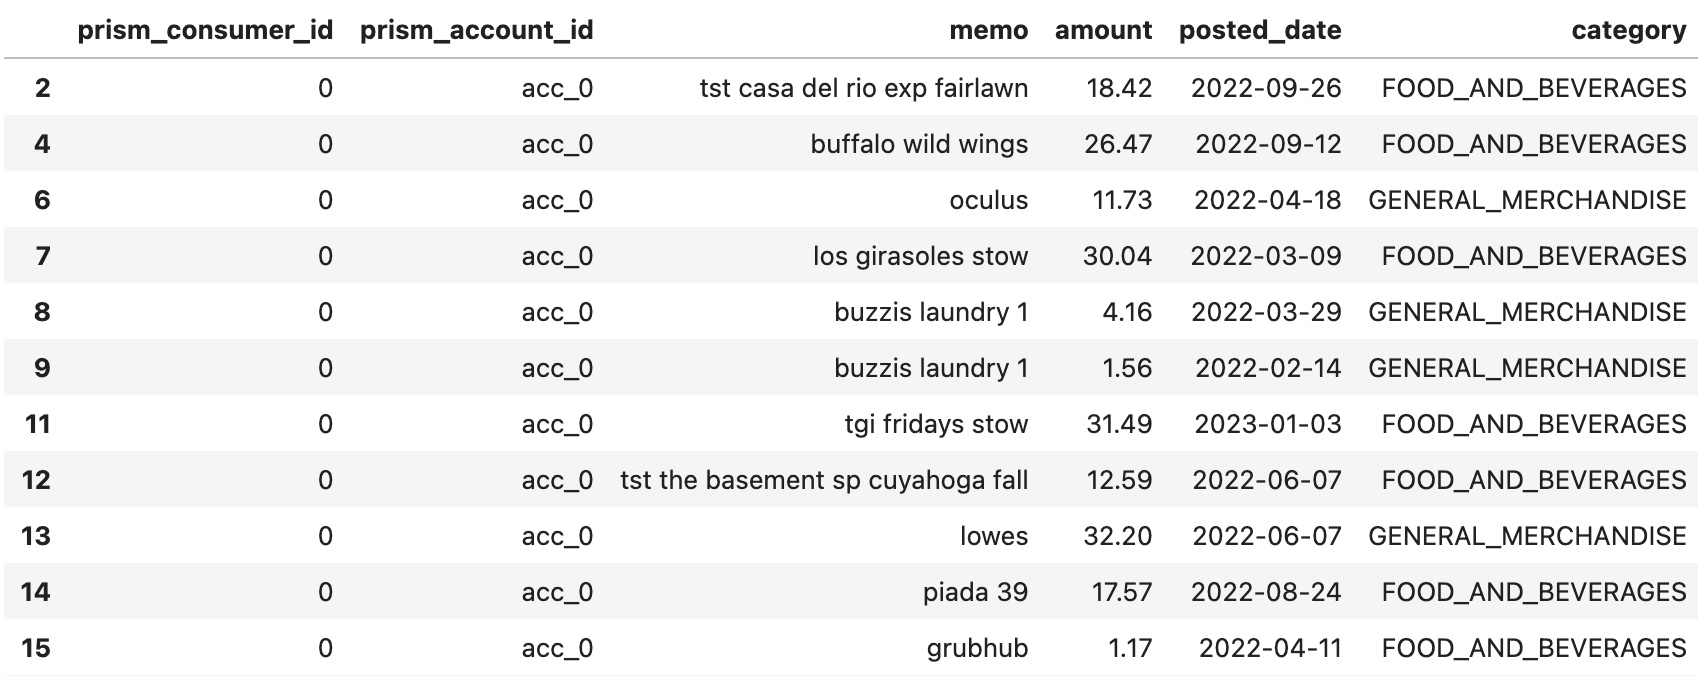
\includegraphics[width=\textwidth]{figure/clean_df.jpeg}
    \caption{This table represents the cleaned memo dataframe, where we applied text preprocessing to ensure consistency across transaction descriptions. By converting to lowercase, removing punctuation, and standardizing certain tokens, we prepared the data for more accurate feature extraction and analysis.}
    \label{fig:clean_memo}
\end{figure}

\subsection{Token Augmentation}
To prepare the transaction data for further analysis and modeling, we enhanced the `memo` field by adding specific tokens based on transaction characteristics. This token augmentation adds additional context about transaction amounts and dates, helping the model learn more meaningful patterns. 

\begin{figure}[h]
    \centering
    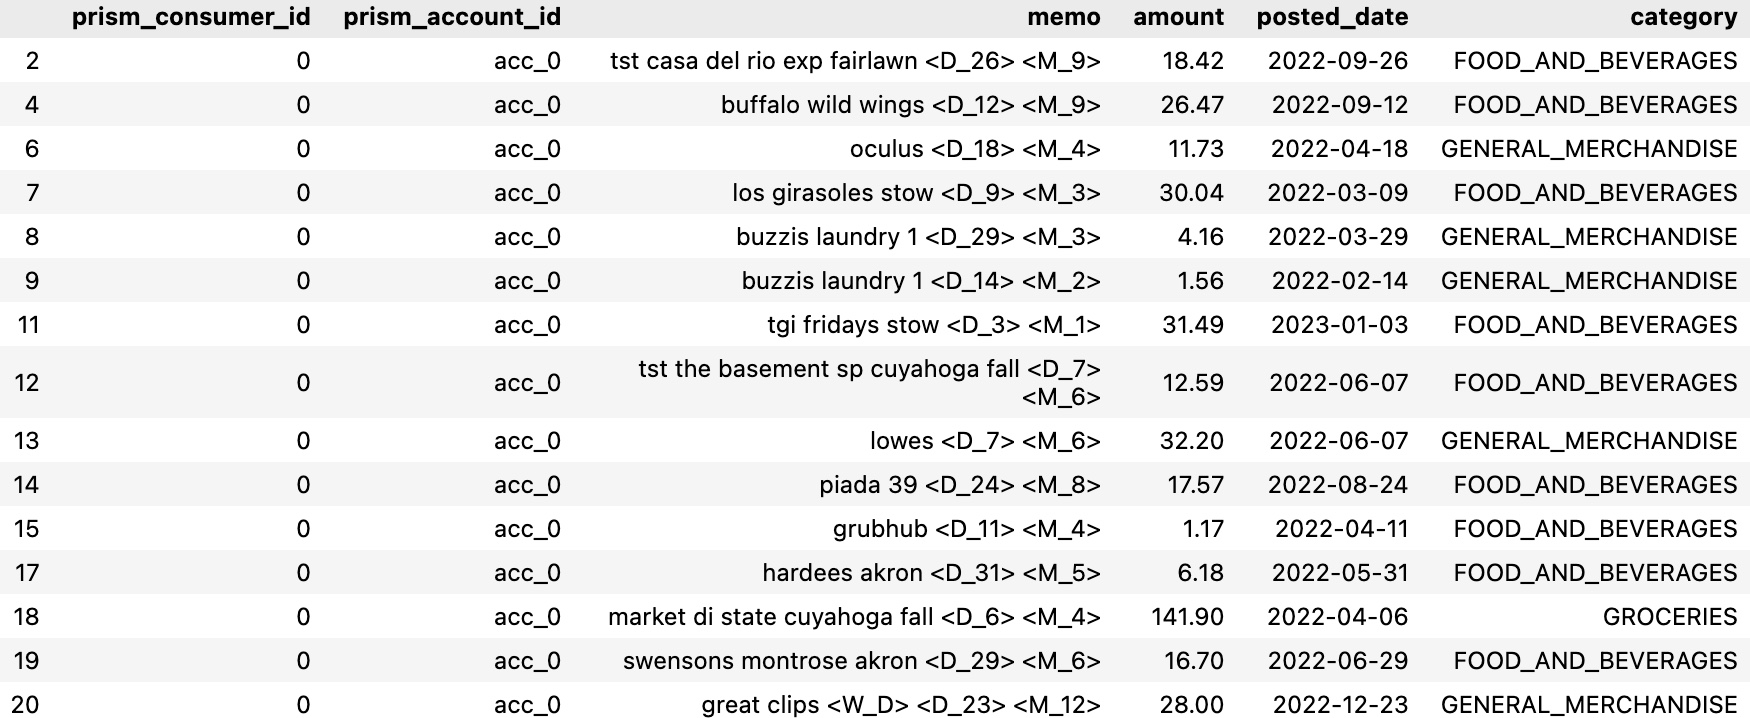
\includegraphics[width=\textwidth]{figure/pre_token.jpeg}
    \caption{This is the transaction data cleaned but not token augmented yet. The \texttt{memo} field contains raw text descriptions without any added tokens.}
    \label{fig:cleaned_data}
\end{figure}

The following steps outline the transformation process:

\begin{enumerate}
    \item \textbf{Whole Dollar Amount Identification}: We added a token \texttt{<W\_D>} to the `memo` field for transactions with whole dollar amounts. This token is useful for identifying transactions that might involve cash withdrawals or ATM transactions, as these are typically in round dollar amounts (e.g., \$20, \$50) since people rarely withdraw amounts with cents.

    \item \textbf{Day of Transaction}: For each transaction's posting date, we generated a day token in the format \texttt{<D\_day>}, where \texttt{day} represents the specific day of the month. This token provides temporal information, which could be helpful for analyzing patterns such as end-of-month or beginning-of-month spending habits.

    \item \textbf{Month of Transaction}: Similarly, we generated a month token in the format \texttt{<M\_month>} (where \texttt{month} is the numerical month) to capture any potential seasonal or monthly trends in spending behavior.

    \item \textbf{Token Augmentation Process}: For each row in the token augmented outflows DataFrame, we concatenated these tokens to the `memo` field:

    \begin{verbatim}
    memo = memo + whole_dollar_amount_token + day_token + month_token
    \end{verbatim}

    where \texttt{whole\_dollar\_amount\_token}, \texttt{day\_token}, and \texttt{month\_token} represent the applicable tokens based on each transaction's attributes.

\end{enumerate}

\begin{figure}[h]
    \centering
    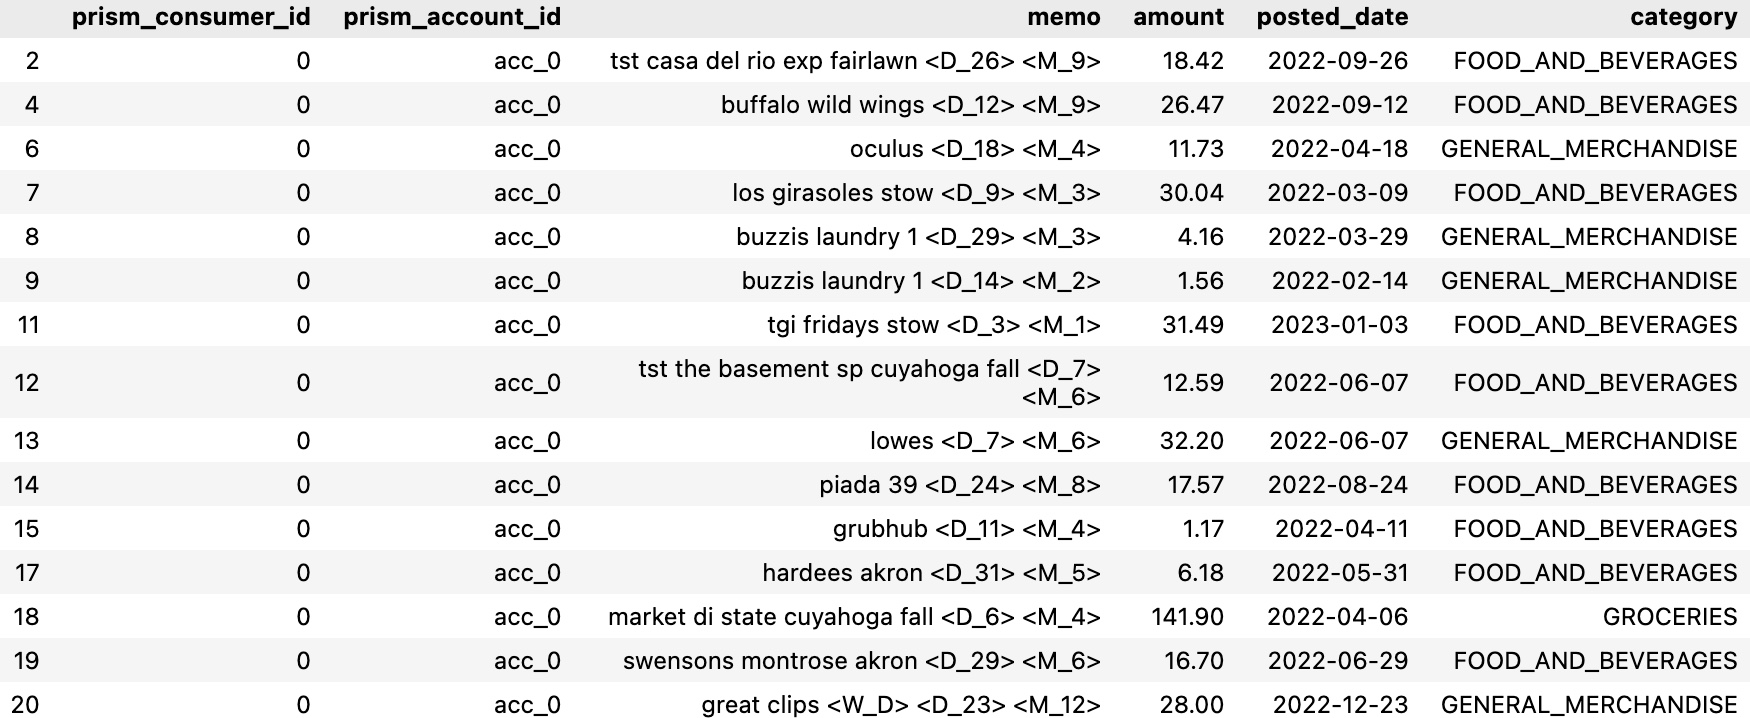
\includegraphics[width=\textwidth]{figure/post_token.jpeg}
    \caption{Transaction data after token augmentation. The \texttt{memo} field has specific tokens added: \texttt{<D\_day>} representing the day of the transaction, \texttt{<M\_month>} representing the month, and \texttt{<W\_D>} indicating a whole dollar amount.}
    \label{fig:token_augmented_data}
\end{figure}


\subsection{Logistic Regression with TF-IDF Vectorization}

To classify transaction categories based on the `memo` text field, we first used a Logistic Regression model with TF-IDF vectorization. This approach transforms the raw text data into numerical features, allowing the model to use term frequency patterns for classification.

\subsubsection{TF-IDF Vectorization}
We employed a TF-IDF (Term Frequency-Inverse Document Frequency) vectorizer to convert text data into a matrix of features. We configured the vectorizer with the following parameters:
\begin{itemize}
    \item \textbf{max\_features=5000}: We set the maximum number of features to 5,000, so we are only using the 5,000 most important terms (based on term frequency and relevance).
    \item \textbf{max\_df=0.95}: We ignored terms that appear in more than 95\% of documents.
    \item \textbf{min\_df=5}: We ignored terms that appear in fewer than 5 documents.
\end{itemize}

We fit the TF-IDF vectorizer on the training data, then applied it to the test data.

\subsubsection{Logistic Regression Model}
For classification, we selected Logistic Regression due to its simplicity and effectiveness in handling high-dimensional text-based data. We configured the model with the following hyperparameters:
\begin{itemize}
    \item \textbf{solver='saga'}: We chose the `saga` solver because it is efficient for large datasets and supports L2 regularization, which helps prevent overfitting by penalizing large coefficients.
    \item \textbf{max\_iter=200}: We set the maximum number of iterations to 200 to ensure convergence.
    \item \textbf{n\_jobs=-1}: We set `n\_jobs` to -1, so that training process would utilize all available CPU cores, running in parallel to improve computational efficiency.
\end{itemize}

This configuration of our Logistic Regression model resulted in a 96.15\% accuracy on the test set.

\subsection{Random Forest with TF-IDF Vectorization}
We also implemented a Random Forest model with TF-IDF vectorization to take on a more complex approach to transaction classification.

\subsubsection{TF-IDF Vectorization}
Similar to the Logistic Regression approach, we utilized TF-IDF to transform the `memo` text into features. We configured the vectorizer with the following parameters:
\begin{itemize}
    \item \textbf{max\_features=2000}: We limited the number of features to 2,000
    \item \textbf{max\_df=0.95}: Similar to the Logistic Regression model, we ignored terms that appear in more than 95\% of documents.
    \item \textbf{min\_df=5}: Similar to the Logistic Regression model, we excluded terms that appear in fewer than 5 documents.
\end{itemize}

\subsubsection{Random Forest Model}
We configured the Random Forest model with the following hyperparameters:
\begin{itemize}
    \item \textbf{n\_estimators=100}: We set the model to use 100 trees (estimators).
    \item \textbf{max\_depth=60}: We restricted the maximum depth of each tree to 60 levels.
    \item \textbf{n\_jobs=-1}: Similar to the Logistic Regression model, we set `n\_jobs` to -1 to leverage all available CPU cores and allow the training process to run in parallel.
\end{itemize}

The Random Forest model achieved an accuracy of 84.28\% on the test set, which was lower than the Logistic Regression model.


\section{Results}
\subsection{Logistic Regression with TF-IDF Vectorization}

The Logistic Regression model with TF-IDF vectorization achieved strong performance in classifying transaction categories. The key metrics used to evaluate the model were overall accuracy, ROC-AUC scores for each category, per-category accuracy, and a confusion matrix.

\subsubsection{Overall Accuracy}
The Logistic Regression model achieved an overall accuracy of 96.15\% on the test set, indicating its effectiveness in distinguishing between different transaction categories based on the tokenized `memo` text.

\subsubsection{ROC-AUC Scores}
To assess the model’s ability to distinguish between each category in a one-vs-all setting, we calculated the ROC-AUC score for each category. Table \ref{table:roc_auc_scores_logreg} provides the ROC-AUC scores for all categories. The high ROC-AUC scores, particularly in categories like \texttt{GROCERIES}, \texttt{FOOD\_AND\_BEVERAGES}, and \texttt{MORTGAGE}, reflect the model's strong performance across multiple categories.

\begin{table}[h]
    \centering
    \begin{tabular}{ll}
        \hline
        \textbf{Category} & \textbf{ROC-AUC Score} \\
        \hline
        EDUCATION & 0.9937 \\
        FOOD\_AND\_BEVERAGES & 0.9956 \\
        GENERAL\_MERCHANDISE & 0.9956 \\
        GROCERIES & 0.9981 \\
        MORTGAGE & 1.0000 \\
        OVERDRAFT & 0.9999 \\
        PETS & 0.9986 \\
        RENT & 0.9969 \\
        TRAVEL & 0.9983 \\
        \hline
    \end{tabular}
    \caption{ROC-AUC Scores for Each Transaction Category in Logistic Regression Model}
    \label{table:roc_auc_scores_logreg}
\end{table}

\subsubsection{Per-Category Accuracy}
We also evaluted the model’s accuracy for each category individually, as shown in Table \ref{table:category_accuracy_logreg}. High per-category accuracy, especially for categories such as \texttt{OVERDRAFT}, \texttt{MORTGAGE}, and \texttt{RENT}, indicates the model's reliability in classifying certain types of transactions with precision.

\begin{table}[h]
    \centering
    \begin{tabular}{ll}
        \hline
        \textbf{Category} & \textbf{Accuracy} \\
        \hline
        GENERAL\_MERCHANDISE & 0.8991 \\
        OVERDRAFT & 0.9998 \\
        EDUCATION & 0.9967 \\
        TRAVEL & 0.9838 \\
        RENT & 0.9984 \\
        MORTGAGE & 0.9993 \\
        PETS & 0.9960 \\
        FOOD\_AND\_BEVERAGES & 0.8476 \\
        GROCERIES & 0.9649 \\
        \hline
    \end{tabular}
    \caption{Per-Category Accuracy for Logistic Regression Model}
    \label{table:category_accuracy_logreg}
\end{table}

\subsubsection{Confusion Matrix}
The confusion matrix for the Logistic Regression model (Figure \ref{fig:log_reg_confusion}) shows the model's classification performance across categories. The matrix illustrates the high precision in categories like \texttt{OVERDRAFT} and \texttt{MORTGAGE}, with fewer misclassifications across these categories. 

\begin{figure}[h]
    \centering
    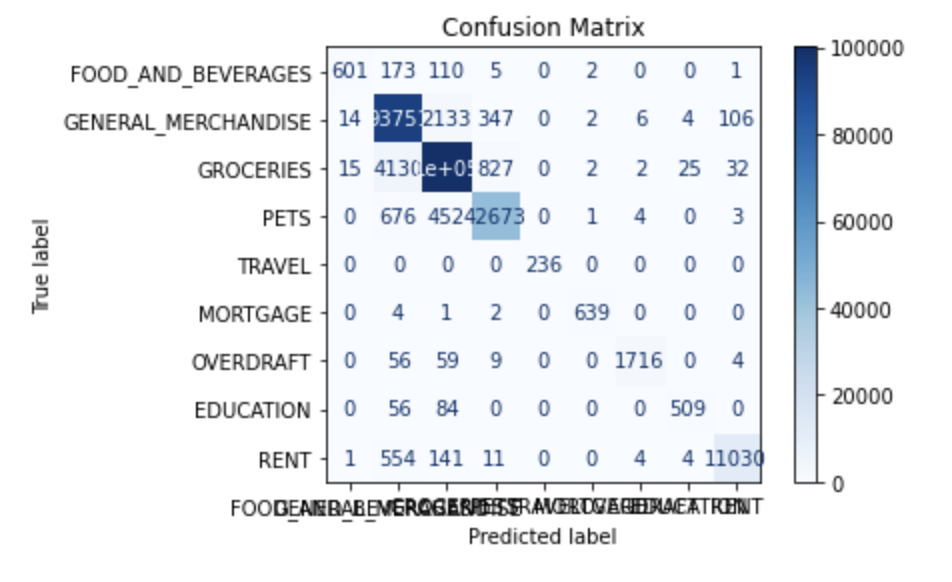
\includegraphics[width=0.8\textwidth]{figure/log_reg_confusion.png}
    \caption{Confusion Matrix for the Logistic Regression Model with TF-IDF Vectorization. The matrix shows true versus predicted labels.}
    \label{fig:confusion_matrix_logreg}
\end{figure}

\subsection{Random Forest with TF-IDF Vectorization}

Although the Random Forest model with TF-IDF vectorization was a more complex classifier, its performance did not surpass the Logistic Regression model's performance. We used the same evaluation metrics for the Random Forest model (overall accuracy, ROC-AUC scores, per-category accuracy, and the confusion matrix).

\subsubsection{Overall Accuracy}
The Random Forest model achieved an overall accuracy of 84.28\% on the test set.

\subsubsection{ROC-AUC Scores}
The ROC-AUC scores for each category are shown in Table \ref{table:roc_auc_rf}. These scores show that the Random Forest model had high discriminatory power in categories like \texttt{FOOD\_AND\_BEVERAGES} and \texttt{MORTGAGE}, but lower power in others, such as \texttt{EDUCATION} and \texttt{OVERDRAFT}.

\begin{table}[h]
    \centering
    \begin{tabular}{ll}
        \hline
        \textbf{Category} & \textbf{ROC-AUC Score} \\
        \hline
        GENERAL\_MERCHANDISE & 0.6648 \\
        OVERDRAFT & 0.1965 \\
        EDUCATION & 0.1667 \\
        TRAVEL & 0.4826 \\
        RENT & 0.4506 \\
        MORTGAGE & 0.7607 \\
        PETS & 0.3297 \\
        FOOD\_AND\_BEVERAGES & 0.8250 \\
        GROCERIES & 0.7506 \\
        \hline
    \end{tabular}
    \caption{ROC-AUC Scores for Each Transaction Category in Random Forest Model}
    \label{table:roc_auc_rf}
\end{table}

\subsubsection{Per-Category Accuracy}
Table \ref{table:category_accuracy_rf} shows the per-category accuracy of the Random Forest model. Categories such as \texttt{OVERDRAFT}, \texttt{MORTGAGE}, and \texttt{RENT} achieved near-perfect accuracy, whereas categories like \texttt{FOOD\_AND\_BEVERAGES} and \texttt{GENERAL\_MERCHANDISE} had lower accuracy.

\begin{table}[h]
    \centering
    \begin{tabular}{ll}
        \hline
        \textbf{Category} & \textbf{Accuracy} \\
        \hline
        GENERAL\_MERCHANDISE & 0.8991 \\
        OVERDRAFT & 0.9998 \\
        EDUCATION & 0.9967 \\
        TRAVEL & 0.9838 \\
        RENT & 0.9984 \\
        MORTGAGE & 0.9993 \\
        PETS & 0.9960 \\
        FOOD\_AND\_BEVERAGES & 0.8476 \\
        GROCERIES & 0.9649 \\
        \hline
    \end{tabular}
    \caption{Per-Category Accuracy for Random Forest Model}
    \label{table:category_accuracy_rf}
\end{table}

\subsubsection{Confusion Matrix}
The confusion matrix for the Random Forest model (Figure \ref{fig:confusion_matrix_rf}) provides insights into its classification performance. Misclassifications are more prevalent in categories like \texttt{FOOD\_AND\_BEVERAGES} and \texttt{GENERAL\_MERCHANDISE}. This pattern suggests that the Random Forest model struggled to distinguish some categories with high similarity in text patterns.

\begin{figure}[h]
    \centering
    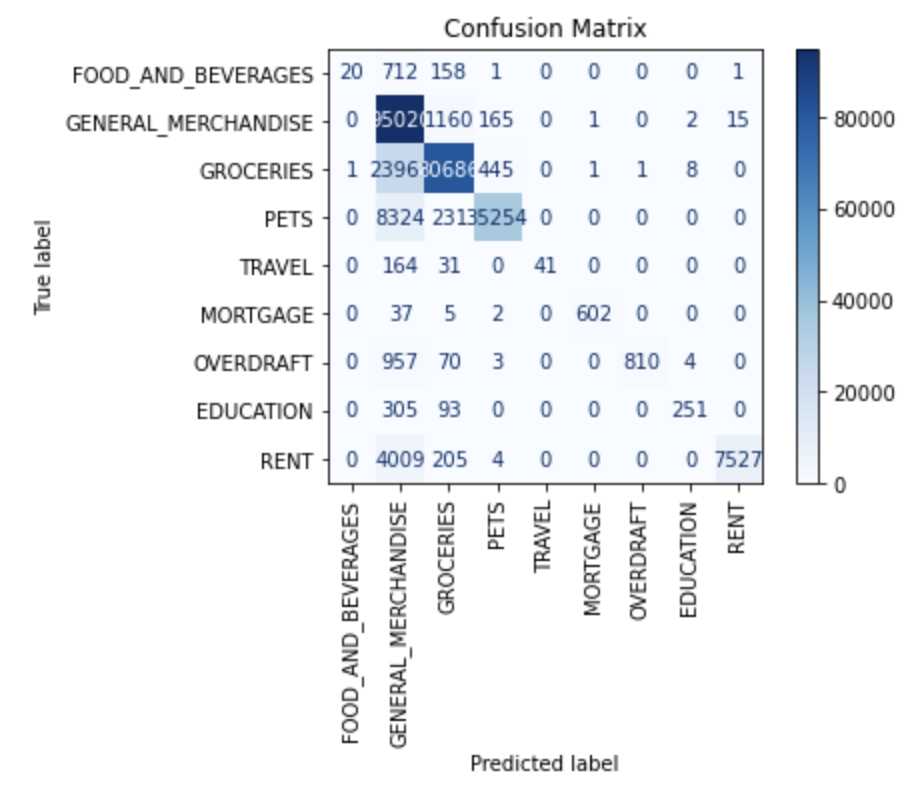
\includegraphics[width=0.8\textwidth]{figure/random_forest_confusion.png}
    \caption{Confusion Matrix for the Random Forest Model with TF-IDF Vectorization.}
    \label{fig:confusion_matrix_rf}
\end{figure}

\section{Discussion}

\subsection{Interpretation of Results}

The Logistic Regression model achieved high accuracy (96.15\%) and strong ROC-AUC scores across most transaction categories, indicating that Logistic Regression, when combined with TF-IDF vectorization, is effective in distinguishing between categories based on term frequency patterns. This performance can largely be attributed to Logistic Regression's ability to handle a large number of features effectively, particularly with the addition of regularization (L2 penalty) using the \texttt{saga} solver. The model's simplicity and its capacity to generalize well without overfitting make it a suitable choice for text-based classification tasks, such as categorizing transaction memos into relevant categories.

Although the Random Forest model is more complex, it achieved a lower overall accuracy of 84.28\% and had mixed performance across categories. While it performed well in certain categories, such as \texttt{OVERDRAFT} and \texttt{MORTGAGE}, it struggled in others, such as \texttt{EDUCATION} and \texttt{GENERAL\_MERCHANDISE}. This discrepancy suggests that model complexity alone does not ensure better performance, particularly for high-dimensional data.

\subsection{Model Comparison}

The likely reason for Random Forest’s lower performance lies in its sensitivity to high-dimensional, sparse data. Random Forest models work best with dense features and can struggle with the many zero-valued features produced by TF-IDF vectorization. In contrast, Logistic Regression’s performance demonstrates that it can handle sparse, high-dimensional data effectively due to its simple, linear structure and the use of regularization to prevent overfitting.

The results indicate that Logistic Regression outperformed Random Forest in both overall accuracy and category-specific ROC-AUC scores. Additionally, the confusion matrices for each model reveal that Logistic Regression made fewer misclassifications, with fewer off-diagonal elements overall compared to the Random Forest model. This finding aligns with the accuracy and ROC-AUC scores, reinforcing the suitability of Logistic Regression with TF-IDF for this task.

\subsection{Limitations}

A primary challenge in text-based classification is managing high-dimensional sparse data effectively. Although Logistic Regression performed well with TF-IDF features, the use of alternative feature extraction methods, such as word embeddings (e.g., Word2Vec or GloVe), could be explored to capture more semantic meaning between words. For the Random Forest model, the high feature sparsity from TF-IDF may have impacted its performance, as Random Forest models typically perform better with dense feature spaces.

\subsection{Potential Improvements}

For Random Forest, addressing feature sparsity by grouping similar words or applying dimensionality reduction techniques, such as Principal Component Analysis (PCA) or Truncated Singular Value Decomposition (SVD), could enhance performance. Additionally, fine-tuning hyperparameters for both models may yield further improvements. For Logistic Regression, experimenting with different regularization strengths or solvers might yield marginal gains. For Random Forest, increasing the number of trees or experimenting with larger maximum depths could enhance performance, though these adjustments may require more computational resources.

Given the mixed results of Random Forest, exploring other models specifically designed for text classification could provide further insight. Support Vector Machines (SVMs), known for their effectiveness on high-dimensional, sparse data, might be a promising alternative for this classification task.

\subsection{Future Work}

Future work could focus on implementing different models and feature engineering techniques to improve classification performance. Also, performing a more extensive hyperparameter search for both Logistic Regression and Random Forest could further optimize each model’s accuracy.

Further understanding the misclassified categories could also provide insights into what the models do not capture effectively.






%%%%%%%%%%%%%%%%%%%%%%%%%%%%%%%%%%%%%%%%%%%%%%%%%%%%%%%%
%%%% Reference / Bibliography
%%%%%%%%%%%%%%%%%%%%%%%%%%%%%%%%%%%%%%%%%%%%%%%%%%%%%%%%

\bibliography{reference}
\bibliographystyle{style/dsc180bibstyle}

\end{document}
